% !TEX root = ../thesis-example.tex
%
\chapter{Resultados}
\label{Resultados}




\section{Resultado del cálculo de entropías}

Se usaron los datos de la base etiquetados como DJJA para la obtención de las siguientes gráficas. 





\begin{figure}
	\centering
	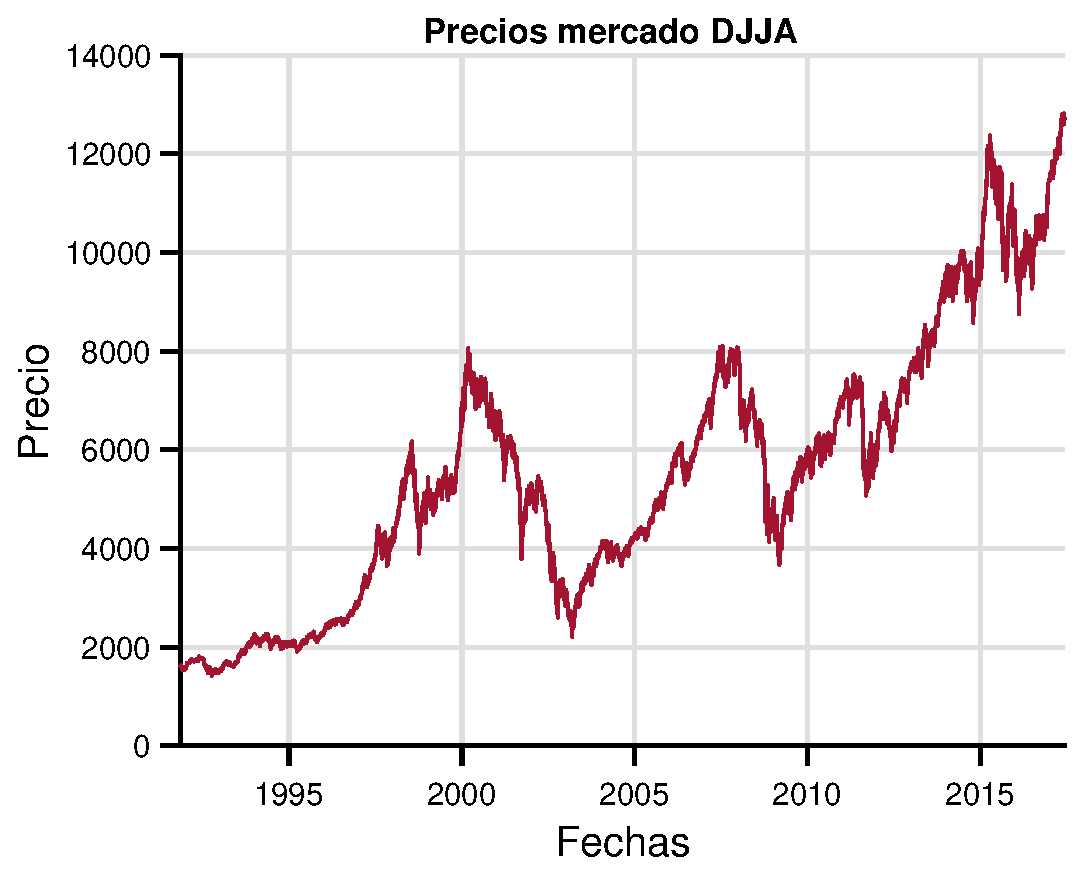
\includegraphics[width=0.7\linewidth]{figures/precioseps}
	\caption{. Evolución temporal de los precios en el mercado DJJA.}
	\label{precioseps}
\end{figure}

En la figura  \ref{precioseps} se tienen los precios en el mercado y su evolución en el tiempo, tal como se muestran dichos precios no se les ha aplicado ningún filtro de media móvil ni ninguna suavización de la curva. Además, entre el año 2000 y 2005, se aprecia una caída en el precio, mismo que tiene impacto al estudiar la entropía.

\begin{figure}
	\centering
	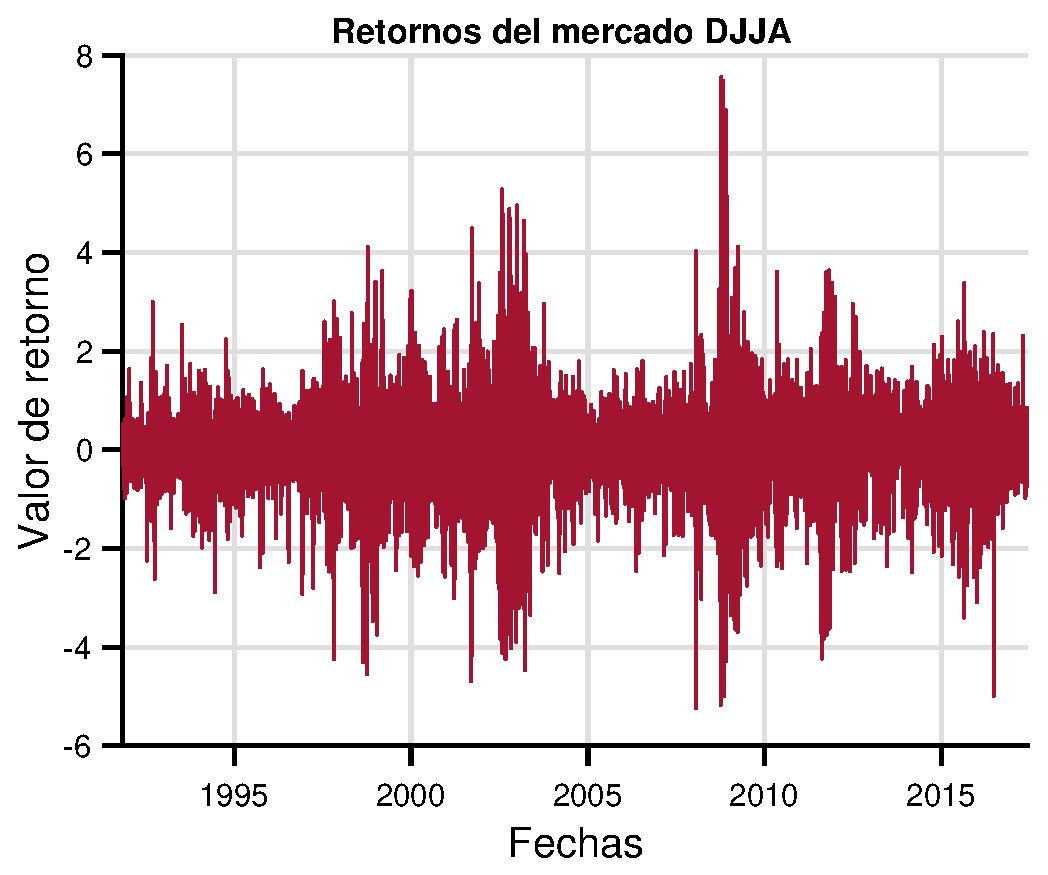
\includegraphics[width=0.7\linewidth]{figures/onlyreturnseps}
	\caption{Retornos para el mercado DJJA.}
	\label{onlyreturnseps}
\end{figure}

Se calcularon lo retornos como se explica en la sección Metodología aplicando el algoritmo de la figura  \ref{diagramaentropia1}. En la figura \ref{onlyreturnseps} se aprecia que los retornos fluctúan entorno a una media de valor cero. Sin embargo se aprecia que existen mínimos en el valor del retorno, como es el caso del segundo mínimo, que además es el mínimo global de todos los retornos.


\begin{figure}
	\centering
	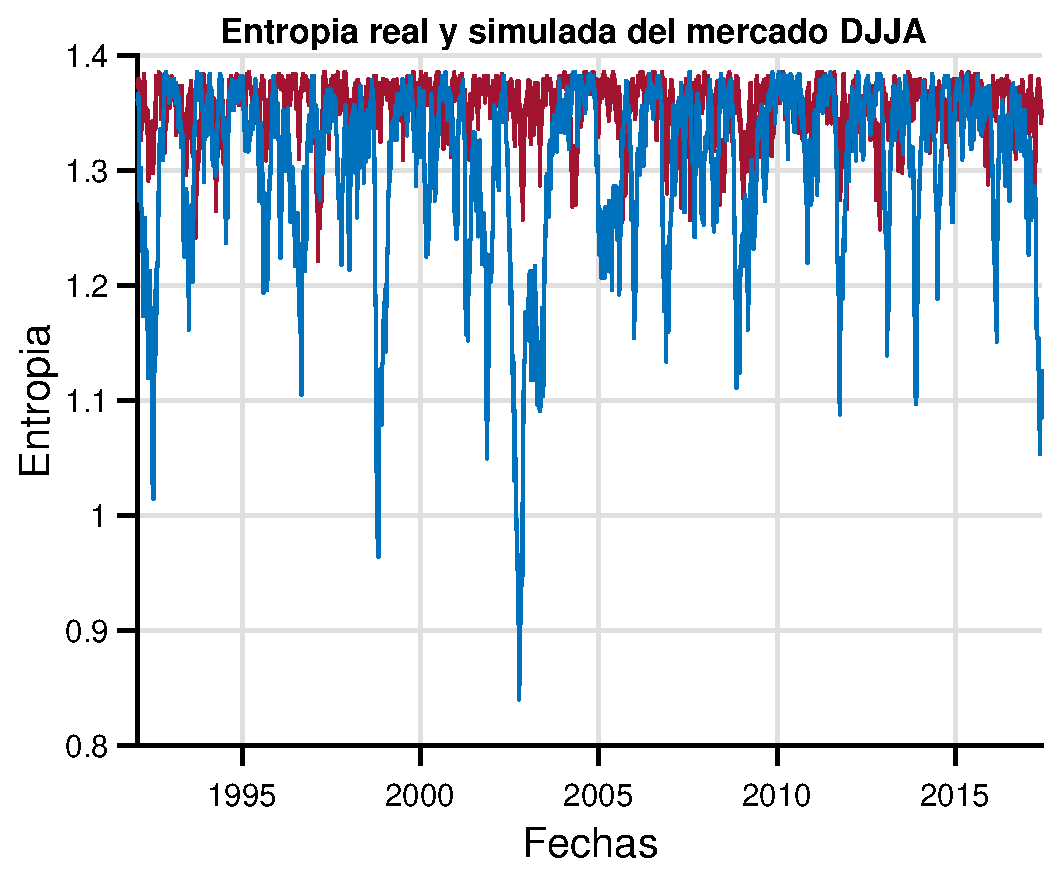
\includegraphics[width=0.7\linewidth]{figures/onlyentropyeps}
	\caption{Entropía para un mercado simulado y un mercado eficiente. Mercado real DJJA (linea azul) y mercado eficiente DJJA (linea roja).}
	\label{onlyentropyeps}
\end{figure}


En la figura \ref{onlyentropyeps} se observa que la entropía posee valores mínimos en la misma fecha (dd/mm/yyyy) del segundo mínimo que muestra el gráfico de los precios (Ver Figura \ref{precioseps}). Un mínimo es observado cuando varias fechas consecutivas el precio es más bajo, resultando el valor de retorno negativo. 




\begin{figure}
	\centering
	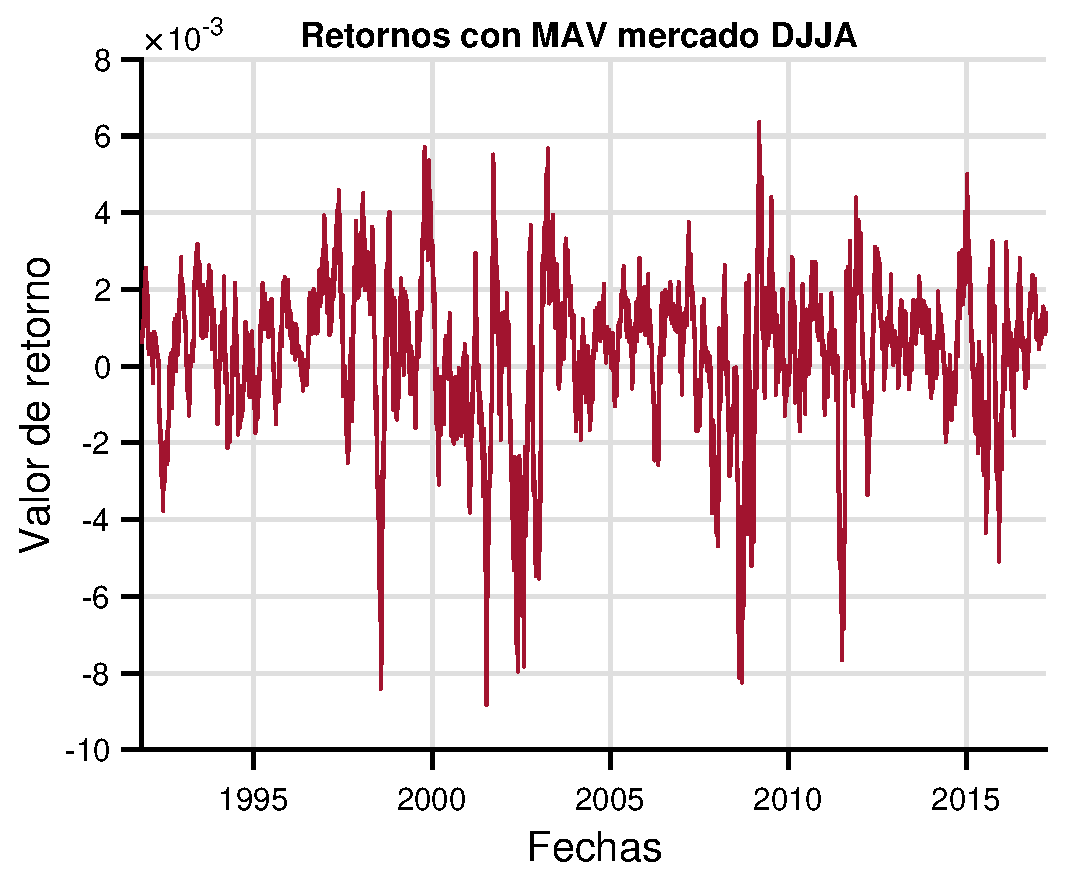
\includegraphics[width=0.7\linewidth]{figures/MAVreturnseps}
	\caption{Retornos con una media móvil de 50 días aplicada para el mercado DJJA.}
	\label{fig:mavreturnseps}
\end{figure}

En la gráfica \ref{fig:mavreturnseps} se puede apreciar que la representación de los datos es menos conglomerada debido a que se aplicó una ventana de 50 días. Este filtrado de datos permite que la gráfica conserve su comportamiento pero que sea fácil identificar puntos de interés.

\begin{figure}
	\centering
	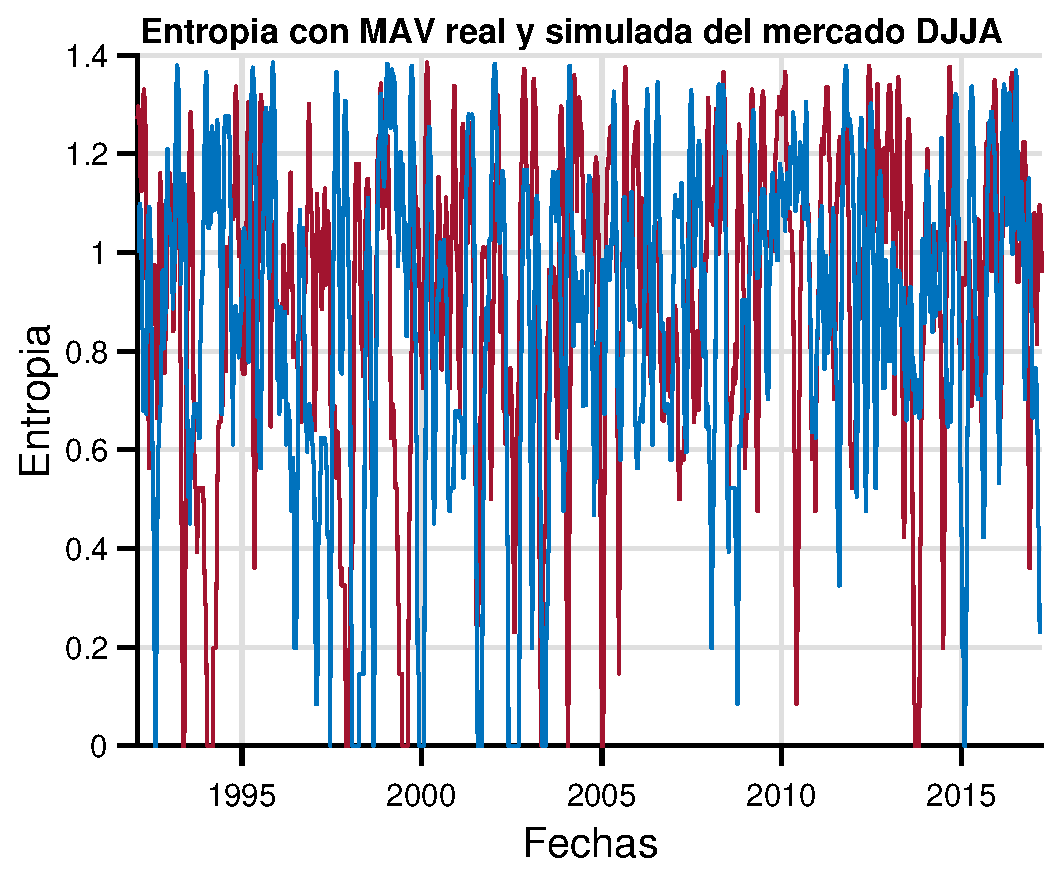
\includegraphics[width=0.7\linewidth]{figures/MAVentropy}
	\caption{Entropia del mercado real DJJA (linea azul) y un la simulacion de un mercado ideal DJJA (linea roja) con aplicación de medias móviles.}
	\label{fig:maventropy}
\end{figure}

En la gráfica de comparación (Ver figura \ref{fig:maventropy} ) entre la entropía del mercado real y la entropía del mercado simulado se tiene que cuando se simulan los retornos y se les aplica un filtro de media móvil, el cálculo de la entropía muestra que hay mínimos de la entropía con valor cero. Los retornos de datos reales muestran un comportamiento similar ya que hay más de un punto en que la entropía mínima también es cero.